\begin{definition}
  В аффиной системе координат общее уравнение линии второго порядка имеет вид:  
  \begin{equation}
    \label{eq:fig_common}
    F(x,\, y) = \underbrace{a_{11}x^2 + a_{22}y^2}_{\text{квадратичная часть}} + 
  \underbrace{2a_{12}xy + 2a_{10}x + 2a_{20}y}_{\text{линейная часть}} + a_{00} = 0,
  \end{equation}
  в котором коэффициенты "--- любые действительные числа, причем $a_{11},\, a_{12}, \, a_{22}$ не равны одновременно нулю.
\end{definition}

Уравнение \ref{eq:fig_common} можно записать в виде:
$$
  F(x, \, y) = \begin{pmatrix} x & y \end{pmatrix} \; \begin{pmatrix}
    a_{11} & a_{12} \\
    a_{21} & a_{22}
  \end{pmatrix} \; \begin{pmatrix} x \\ y \end{pmatrix} + 2 \begin{pmatrix} a_{10} & a_{20} \end{pmatrix} \begin{pmatrix} x \\ y \end{pmatrix} + a_{00} = 0
$$

\begin{lemma}
  Подходящим поворотом осей координат можно добиться того, что $a_{12}'= 0$, где штрих означает соответствующий коэффициент уравнения кривой второго порядка в новой системе координат.
\end{lemma}
\begin{Proof}
  Рассмотрим поворот: 
  $$
  \begin{pmatrix} x \\ y \end{pmatrix} = 
  \begin{pmatrix}
    \cos \varphi & -\sin \varphi \\
    \sin \varphi & \cos \varphi
  \end{pmatrix} \begin{pmatrix} x' \\ y' \end{pmatrix}
  $$
  Тогда 
  \begin{gather*} F(x', \, y') = a_{11}(x'\, \cos \varphi - y' \, \sin \varphi)^2 + a_{22} (x' \, \sin \varphi + y'\, \cos \varphi)^2 + \\ + 2a_{12}(x' \, \cos \varphi - y' \, \sin \varphi)(x' \, \sin \varphi + y'\, \cos \varphi)+
  2a_{10}(x'\, \cos \varphi - y' \, \sin \varphi) + \\ + 2a_{20}(x' \, \sin \varphi + y' \, \cos \varphi) + a_{00} = 0 
  \end{gather*}
  Коэффициент при $2x'\, y'$, то есть $a_{12}'$ равен
  \begin{gather*}
    a_{12}' = -a_{11}\cos \varphi \sin \varphi + a_{12}(\cos^2 \varphi - \sin^2 \varphi) + a_{22}\cos \varphi \sin \varphi  = 0 \\
    a_{12}\cos 2\varphi = \frac{1}{2} \sin 2\varphi (a_{11} - a_{22}) \\
    \operatorname{tg} 2 \varphi = \frac{2a_{12}}{a_{11} - a_{22}} 
  \end{gather*}
\end{Proof}
Выполнив поворот оси на угол $\varphi$, многочлен $F$ примет вид:
\begin{equation}
  \label{eq:fig_del12}
  F'(x', \, y') = \lambda_1 x'^{\, 2} + \lambda_2 y'^{\, 2} + 2b_1x' + 2b_2y' + b_0 = 0
\end{equation}
\begin{lemma}
  Многочлен вида \ref{eq:fig_del12} параллельным переносом приводится к одному из следующих видов:
  \begin{enumerate}
    \item \begin{equation}
      \label{eq:lemma_1}
      F'' = \lambda_1(x'')^2 + \lambda_2(y'')^2 + \tau, ~ (\lambda_1,\, \lambda_2 \neq 0)
    \end{equation}
    \item \begin{equation}
      \label{eq:lemma_2}
      F'' = \lambda_2(y'')^2 + 2b_1x'', ~ (\lambda_2, \, b_1 \neq 0)
    \end{equation}
      \item \begin{equation}
        \label{eq:lemma_3}
        F'' = \lambda_2(y'')^2 + \tau, ~ (\lambda_2 \neq 0)
      \end{equation}
  \end{enumerate}
\end{lemma}
\begin{Proof}
  \begin{enumerate}
    \item $\lambda_1, \, \lambda_2 \neq 0$
    \begin{gather*}
      F'(x', \, y') = \lambda_1 x'^{\, 2} + \lambda_2 y'^{\, 2} + 2b_1x' + 2b_2y' + b_0 =\\
      =\lambda_1 \Bigl(\underbrace{x' + \frac{b_1}{\lambda_1}}_{x''}\Bigr)^2 + \lambda_2\Bigl(\underbrace{y' + \frac{b_2}{\lambda_2}}_{y''}\Bigr)^2 + \Bigl(\underbrace{b_0 - \frac{b_1^2}{\lambda_1} - \frac{b_2^2}{\lambda_2}}_{\tau}\Bigr) = \\
      = \lambda_1(x'')^2 + \lambda_2(y'')^2 + \tau,
    \end{gather*}
  \end{enumerate}
  \item $\lambda_1 = 0, \; \lambda_2 \neq 0$ (если наоборот, то поменяем координаты местами). Возможны два случая:
  \begin{enumerate}
    \item если $b_1 \neq 0$, то 
    \begin{gather*}
      F'(x', \, y') = \lambda_2 y'^{\, 2} + 2b_1x' + 2b_2y' + b_0 =\\
      = \lambda_2\Bigl(y' + \frac{b_2}{\lambda_2} \Bigr)^2 + 2b_1x' + \Bigl(b_0 - \frac{b_2^2}{\lambda_2}\Bigr) = \\
      = \lambda_2\Bigl(\underbrace{y' + \frac{b_2}{\lambda_2}}_{y''} \Bigr)^2 + 2b_1\Bigl(\underbrace{x' + \frac{1}{2b_1}\bigl(b_0 - \frac{b_2^2}{\lambda_2}\bigr)}_{x''}\Bigr) = \\
      = \lambda_2(y'')^2 + 2b_1x''
    \end{gather*}
    \item если $b_1 = 0$, то
    \begin{gather*}
      F'(x', \, y') = \lambda_2 y'^{\, 2} + b_2y' + b_0 = \\
      = \lambda_2\Bigl(\underbrace{y' + \frac{b_2}{\lambda_2}}_{y''}\Bigr)^2 + \Bigl(\underbrace{b_0 - \frac{b_2^2}{\lambda_2}}_{\tau}\Bigr) = \\
      = \lambda_2(y'')^2 + \tau
    \end{gather*}
  \end{enumerate}
\end{Proof}

\begin{theorem}
  \label{theorem:second}
  Для любой кривой второго порядка существует прямоугольная система координат, в которой она имеет один из следующих видов (называемых каноническими уравнениями):
  \begin{enumerate}
    \item $\frac{x^2}{a^2} + \frac{y^2}{b^2} = 1, ~(a \geq b > 0),$ эллипс 
    \item  $\frac{x^2}{a^2} + \frac{y^2}{b^2} = -1, ~(a \geq b > 0),$ мнимый эллипс 
    \item  $\frac{x^2}{a^2} - \frac{y^2}{b^2} = 1, ~(a \geq b > 0),$ гипербола
    \item  $\frac{x^2}{a^2} - \frac{y^2}{b^2} = 0, ~(a \geq b > 0),$ пара пересекающихся прямых
    \item $\frac{x^2}{a^2} + \frac{y^2}{b^2} = 0, ~(a \geq b > 0),$ пара пересекающихся мнимых прямых 
    \item $y^2 = 2px, ~ (p > 0),$ парабола
    \item $y^2 - a^2 = 0, ~ (a > 0),$ пара параллельных прямых
    \item $y^2 + a^2 = 0, ~ (a > 0),$ пара мнимых параллельных прямых
    \item $y^2 = 0$ пара совпадающих прямых
  \end{enumerate}
\end{theorem}

Рассмотрим различные равенства \ref{eq:lemma_1}--\ref{eq:lemma_3}:
\begin{enumerate}
  \item $F'' = \lambda_1(x'')^2 + \lambda_2(y'')^2 + \tau, ~ (\lambda_1,\, \lambda_2 \neq 0)$
  \begin{enumerate}[label = \alph*)]
    \item $\lambda_1, \, \lambda_2$ "--- одного знака, $\tau$ "--- противоположного. Получаем уравнение эллпипса.
    \item $\lambda_1, \, \lambda_2, \, \tau$ "--- одного знака. Получаем уравнение мнимого эллипса.
    \item $\lambda_1, \, \lambda_2$ "--- одного знака, $\tau = 0$. Пара пересекающихся мнимых прямых.
    \item $\lambda_1, \, \lambda_2$ "--- разных знаков, $\tau \neq 0$. Гипербола
    \item $\lambda_1, \, \lambda_2$ "--- разных знаков, $\tau = 0$. Пара пересекающихся прямых.
  \end{enumerate}
  \item $F'' = \lambda_2(y'')^2 + 2b_1x'', ~ (\lambda_2, \, b_1 \neq 0)$. Парабола
  \item $ F'' = \lambda_2(y'')^2 + \tau, ~ (\lambda_2 \neq 0)$
  \begin{enumerate}[label = \alph*)]
    \item $\tau < 0$. Пара параллельных прямых.
    \item $\tau > 0$. Пара мнимых параллельных прямых.
    \item $\tau = 0$. Пара совпадающих прямых.
  \end{enumerate}
\end{enumerate}

\subsection*{Эллипс}
Эллипсом по теореме \ref{theorem:second} была названа линия, которая в некторой прямоугольной системе координат определяется каноническим уравнением:
\begin{equation}
  \label{eq:ellipse}
  \frac{x^2}{a^2} + \frac{y^2}{b^2} = 1
\end{equation}
Из уравнения \ref{eq:ellipse} следует, что для всех точек эллипса $\mathopen|x\mathclose| \leq a$ и $\mathopen|y\mathclose| \leq b$
\begin{figure}[H]
  \centering
  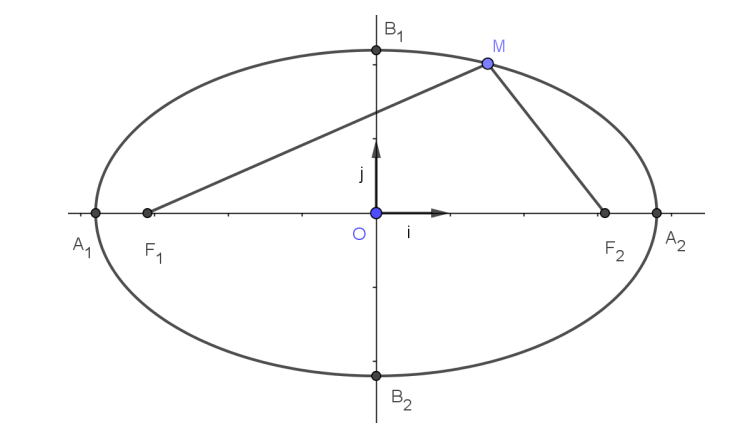
\includegraphics[width = \textwidth]{images/second_ellipse.png}
  \caption{Эллипс. $OA_2 = OA_1 = a, ~ OB_1 = OB_2 = b$}
  \label{fig:ellipse} 
\end{figure}

Точки, имеющие координаты $(a,\, 0), \, (a,\, 0), \, (0,\, b), \, (0,\, -b)$ называются \textit{вершинами} эллипса.

С эллипсом связаны две замечательные точки, называемые его \textit{фокусом} (на рисунке \ref{fig:ellipse} отмечены точками $F_1$ и $F_2$). Пусть по определению 
$$
  c^2 = a^2 - b^2
$$
и $c \geq 0$. Тогда точки $F_1$ и $F_2$ имеют координаты $(-c,\, 0)$ и $(c, \, )$ соответственно. Расстояние между фокусами называется \textit{фокальным расстоянием}.

Если $M$ "--- точка эллипса, то отрезки $F_1M$ и $F_2M$ называются \textit{фокальными радиусами} точки $M$. Их длины также называют фокальными радиусами точки $M$. 

Оказывается для того чтобы точка лежала на эллипсе, необходимо и достаточно, чтобы сумма ее расстояний до фокусов равнялась $2a$. 

\begin{Proof}
  Пусть сумма расстояний до фокусов равняется $2a$. Фокальные радиусы точки $M(x,\, y)$ эллипса равны:
  $$
    F_1M = \sqrt{(x + c)^2 + y^2}, ~~ F_2M = \sqrt{(x - c)^2 + y^2}.
  $$
  и $F_1M + F_2M = 2a$. Запишем это выражение в виде:
  $$
    \sqrt{(x + c)^2 + y^2} = 2a - \sqrt{(x - c)^2 + y^2}.
  $$
  Возводя его в квадрат и приводя подобные члены, получим:
  $$
    a\sqrt{(x - c)^2 + y^2} = a^2 - xc.
  $$
  Снова возводя в квадрат, после преобразований получим:
  $$
    \frac{x^2}{a^2} + \frac{y^2}{b^2} = 1,
  $$
  где $b^2  = a^2 - c^2$. Таким образом, $M$ удовлетворяет уравнению \ref{eq:ellipse}.

  Пусть точка $M$ удовлетворяет уравению \ref{eq:ellipse}. Тогда $F_1M = \sqrt{(a + \frac{c}{a}x)^2} = \mathopen|a + \frac{c}{a}x$, $F_2M = \sqrt{(a - \frac{c}{a}x)^2} = \mathopen|a - \frac{c}{a}x\mathclose|$. 

  Так как $\mathopen|x\mathclose| \leq a$, и так как $0 < e = \frac{c}{a} < 1$, то поэтому $a + \frac{c}{a}x > 0, ~ a - \frac{c}{a}x > 0$, поэтому $$
    F_1M = a - \frac{c}{a}x, ~~ F_2M = a + \frac{c}{a}x.
  $$
  Следовательно, $F_1M + F_2M = 2a$.
\end{Proof}

Учитывая это, можно дать определение эллипса:
\begin{definition}
  \textit{Эллипсом} называется множество всех точек плоскости, сумма расстояний каждой из которых до данных точек $F_1$ и $F_2$ равна длине данного отрезка $PQ$, причем $PQ > F_1F_2$.
\end{definition}

Если точки $F_1$ и $F_2$ совпадают, то эллипс является окружностью радиуса $a$. В этом случае фокусы эллипса совпадают с центром окружности. Таким образом, \textit{окружность есть частный случай эллипса}.

Эллипс имеет один центр симметрии и две оси симметрии. Центр симметрии совпадает с серединой фокального отрезка. Прямая, проходящая через фокусы, называется \textit{первой} или \textit{фокальной} осью симметрии, а перпендикулярная к ней ось "--- второй осью симметрии.

Отрезки $2a \, (A_1A_2)$ и $2b \, (B_1B_2)$ называются \textit{большой} и \textit{малой осями} эллипса а $a$ и $b$ "--- \textit{большой} и \textit{малой полуосями} эллипса.

Отношение
$$
  e = \frac{c}{a}
$$ называется \textit{эксцентриситетом} эллипса.

Эксцентриситет равен нулю тогда и только тогда, когда $c = 0$, т.е. когда
эллипс является окружностью. Эксцентриситет эллипса заключен в пределах: $0 < e < 1$. Он характеризует форму эллипса. В самом деле, выразим $\frac{b}{a}$ через эксцентриситет:
$$
  c = ea \implies b^2 = a^2 - c^2 = a^2(1 - e^2) \implies \frac{b}{a} = \sqrt{1 - e^2}.
$$
Отсюда видно, что чем ближе $e$ к $0$, тем ближе $b$ к $a$, т.е. тем ближе эллипс
по форме к окружности. Если же $e$ приближается к $1$, то его малая полуось $b$ приближается к нулю, т.е. эллипс все более вытягивается и в пределе превращается в отрезок.


\begin{definition}
  С эллипсом связаны две замечательные прямые, называемые его \textit{директрисами}. Это две прямые, параллельные  малой оси и отстоящие от нее на расстоянии, равном $\frac{a}{e}$. 
  
  Уравнения директрис $d_1$ и $d_2$ следующие: $x = \pm \frac{a}{e}$.
\end{definition}
Оказывается, для того чтобы точка лежала на эллипсе, необходимо и достаточно, чтобы отношение ее расстояние до фокуса к расстоянию до соответсвтующей директрисы равнялось эксцентриситету эллипса $e$.

Уравнения $x = a \cos t, ~ y = b\sin t ~(0 \leq t \leq 2\pi)$ называются \textit{параметрическими уравнениями эллипса}.

Касательная к эллипсу, заданного уравнением \ref{eq:ellipse}, в точке $(x_0; y_0)$ определяется уравнением:
$$
  \frac{xx_0}{a^2} + \frac{yy_0}{b^2} = 1
$$

\subsection*{Гипербола}
Гиперболой по теореме \ref{theorem:second} была названа линия, которая в некоторой прямоугольной системе координат определяется каноническим уравнением:
\begin{equation}
  \label{eq:hyperbola}
  \frac{x^2}{a^2} - \frac{y^2}{b^2} = 1.
\end{equation}
Из этого уравнения видно, что все точки гиперболы лежат левее точки $(-a,\, 0)$ и правее точки $(a, \, 0)$, называемые \textit{вершинами} гиперболы.

\begin{figure}[H]
  \centering
  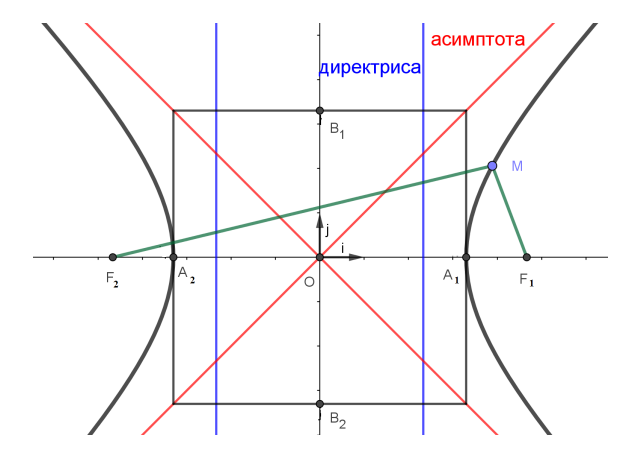
\includegraphics[height = 7cm]{images/second_hyperbola.png}
  \caption{Гипербола. $OA_1 = OA_2 = a$}
  \label{fig:hyperbola}
\end{figure}

Введём число $c$, положив
$$
  c^2 = a^2 + b^2
$$ и $c > 0$. \textit{Фокусами} гиперболы называются точки $F_1$ и $F_2$ с координатами $(c, 0)$ и $(-c, 0)$. Расстояние между ними называется \textit{фокальным расстоянием}.

Если точка $M$ "--- точка данной гиперболы, то отрезки $F_1M$ и $F_2M$ называются \textit{фокальными радиусами} точки $M$. Их длины также называются фокальными радиусами точки $M$.

\begin{theorem}
  Для того чтобы точка $M$ лежала на гиперболе необходимо и достаточно, чтобы разность её расстояний до фокусов по абсолютной величине равнялась $2a$.
\end{theorem}
\begin{Proof}
  $\Rightarrow$ Пусть $M$ удовлетворяет уравнению \ref{eq:hyperbola}. Тогда
    $$
    F_1M = \sqrt{(x - c)^2 + y^2}, ~ F_2M = \sqrt{(x + c)^2 + y^2}.
    $$
    Подставив значение $y^2$ из уравнения \ref{eq:hyperbola} и учитывая, что $c^2 = a^2 + b^2$, получим:
    \begin{gather*}
      F_1M = \sqrt{(\frac{c}{a}x - a)^2} = \mathopen|\frac{c}{a}x - a \mathclose| \\
      F_2M = \sqrt{(\frac{c}{a}x + a)^2} = \mathopen|\frac{c}{a}x + a \mathclose|
    \end{gather*}
    Так как $\mathopen|x\mathclose| \geq a, ~ \frac{c}{a} > 1$, то 
    $$
    \begin{array}{ccc}
      F_1M = \frac{c}{a}x - a, & F_2M = \frac{c}{a}x + a, & \text{при }x > 0 \\
      F_1M = -\frac{c}{a}x + a, & F_2M = -\frac{c}{a}x - a, & \text{при }x < 0 
    \end{array}
    $$
    То есть $\mathopen|F_1M - F_2M\mathclose| = 2a$.

  $\Leftarrow$ Пусть $\mathopen|F_1M - F_2M\mathclose| = 2a$. Тогда
  $$
    \mathopen| \sqrt{(\frac{c}{a}x - a)^2} - \sqrt{(x + c)^2 + y^2} \mathclose| = 2a
  $$
  Запишем это уравнение в виде 
  $$
  \mathopen| \sqrt{(\frac{c}{a}x - a)^2} = \sqrt{(x + c)^2 + y^2} \mathclose| \pm 2a
  $$
  Возводя его в квадрат и приводя подобные члены, получим:
  $$
    \pm a \sqrt{(x - c)^2 + y^2} = a^2 - xc
  $$
  Снова возводя в квадрат, после преобразований получим:
  $$
    \frac{x^2}{a^2} - \frac{y^2}{b^2} = 1
  $$
\end{Proof}
Теперь можно дать определение гиперболы:
\begin{definition}
  \textit{Гиперболой} называется множество всех точек плоскости, абсолютное значение разности расстояний каждой из которых от двух данных точек $F_1$ и $F_2$ равно длине данного отрезка $PQ$, причем $PQ < F_1F_2$.
\end{definition}


Гипербола имеет один центр симметрии и две оси симметрии. Центр симметрии совпадает с серединой фокального отрезка. Прямая, проходящая через фокусы, называется первой или фокальной осью симметрии, а перпендикулярная к ней ось "--- второй или мнимой осью симметрии. Фокальная ось
симметрии пересекает гиперболу в двух точках $A_1$ и $A_2$. Вторая ось симметрии не пересекает гиперболу. Точки $A_1$ и $A_2$ называются вершинами гиперболы, отрезок
$A_1A_2 = 2a$ — \textit{действительной} осью. Отрезок $2b$ — \textit{мнимой} осью. Числа $a$ и $b$
называются соответственно \textit{действительной} и \textit{мнимой полуосями} гипербол.

Гипербола \ref{eq:hyperbola} состоит из двух \textit{ветвей} (правой и левой) и расположена
симметрично относительно осей координат.

Отношение
$$
  e = \frac{c}{a}
$$ называется \textit{эксцентриситетом} гиперболы.

Так как $a < c$, то $e > 1$.

Выясним, как зависит форма гиперболы от её эксцентриситета. Так как $c^2 = a^2 + b^2$ получаем: $\frac{b}{a} =\sqrt{e^2 - 1}$ или $\operatorname{tg}\, \alpha = \sqrt{e^2 - 1}$
где $\alpha$ – угол между осью
абсцисс и асимптотой. Отсюда следует, что больше эксцентриситет, тем больше $\alpha$, т.е. тем больше гипербола <<вытянута>> вдоль своей мнимой оси.

Расстояние от произвольной точки $M(x,y)$ вычисляется:
\begin{itemize}
  \item Если $M$ принадлежит правой ветке: $r_1 = ex - a$, $r_2 = ex + a$.
  \item Если $M$ принадлежит левой ветке: $r_1 = -ex + a$, $r_2 = -ex - a$.
\end{itemize}
В общем виде это можно записать так:
$$
  r_1 = \mathopen|ex - a\mathclose| \text{ и } r_2 = \mathopen|ex + a\mathclose|
$$

\begin{definition}
  \textit{Директрисами гиперболы} называются две прямые, перпендикулярные фокальной оси и отстоящие от центра на расстоянии, равном $\frac{a}{e}$.

  Уравнения директрис $d_1$ и $d_2$ следующие: $x = \pm \frac{a}{e}$.
\end{definition}
Для того, чтобы точка лежала на
гиперболе, необходимо и достаточно, чтобы отношение ее
расстояния до фокуса к расстоянию до соответствующей
директрисы равнялось эксцентриситету $e$.

Гипербола также имеет две асимптоты, уравнения которых $y = \pm \frac{b}{a}x$. На асимптотах лежат диагонали прямоугольника, центр которого совпадает с центром
гиперболы, а стороны равны и параллельны осям гиперболы.

Произведение расстояний от точки гиперболы до асимптот постоянно и равно $\frac{a^2b^2}{a^2 + b^2}$

Гипербола, полуоси которой равны $(a = b)$, называется \textit{равносторонней}. Ее каноническое уравнение имеет вид: $x^2 - y^2 = a^2$.

\begin{definition}
  Гипербола, задаваемая уравнением
  $$
    -\frac{x^2}{a^2} + \frac{y^2}{b^2} = 1
  $$
  называется \textit{сопряженной} с гиперболой, задаваемой с уравнением \ref{eq:hyperbola}. Она пересекает ось $Oy$ в точках $B_1(b,0), \; B_2(-b, 0)$, не пересекает ось $Ox$, так что $a$ "--- ее мнимая полуось, а $b$ "--- действительная.
\end{definition}

Касательная к гиперболе, задаваемая уравнением \ref{eq:hyperbola}, в точке $(x_0; y_0)$ определяется уравнением:
$$
  \frac{xx_0}{a^2} - \frac{yy_0}{b^2} = 1
$$

\subsection*{Парабола}
Параболой по теореме \ref{theorem:second} была названа линия, которая в некоторой прямоугольной системе координат определяется каноническим уравнением:
\begin{equation}
  \label{eq:parabola}
  y^2 = 2px
\end{equation} при условии $p > 0$.

Из уравнения \ref{eq:parabola} вытекает, что для всех точек параболы выполняется $$\begin{cases}
  x \geq 0,& \text{если } p > 0 \\
  x \leq 0,& \text{если } p < 0
\end{cases}$$.
\begin{figure}[H]
  \centering
  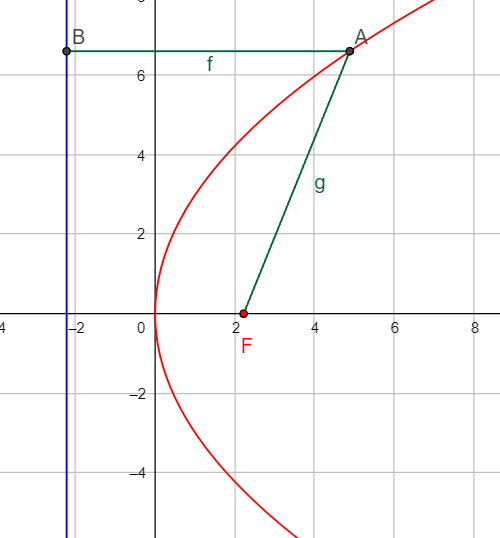
\includegraphics[height = 7cm]{images/second_parabola.png}
  \label{fig:parabola}
\end{figure}

\textit{Фокусом} параболы называется точка $F$ с координатами $(p / 2, 0)$

\textit{Директрисой} параболы называется прямая $d$ с уравнением $x = -\frac{p}{2}$

\begin{theorem}
  Для того, чтобы точка $M$ лежала
  на параболе, необходимо и достаточно, чтобы она была одинаково удалена от фокуса и от директрисы этой параболы.
\end{theorem}
\begin{Proof}
  $\Rightarrow$ Пусть $M$ удовлетворяет уравнению \ref{eq:parabola}. Тогда
  \begin{gather*}
    \rho (M, d) = \mathopen|x + \frac{p}{2}\mathclose| \\
    MF = \sqrt{(x - \frac{p}{2})^2 + y^2} = \\
    = \sqrt{(x - \frac{p}{2})^2 + 2px} = \sqrt{(x + \frac{p}{2})^2} =  \\
    = \mathopen|x + \frac{p}{2}\mathclose| = \rho (M, d)
  \end{gather*}
  $\Leftarrow$ Пусть $M$ одинаково удалена от фокуса и от директрисы параболы:
  $$
    \sqrt{(x - \frac{p}{2})^2 + y^2} = \mathopen|x + \frac{p}{2}\mathclose|
  $$
  Возводя обе части в квадрат, получаем $y^2 = 2px$.
\end{Proof}
Дадим определение параболе.
\begin{definition}
  Параболой называется множество всех точек плоскости, расстояние каждой из которых до данной точки равно расстоянию до данной прямой $d$, не проходящей через точку $F$.
\end{definition}
Парабола имеет одну ось симметрии, которая совпадает, при таком выборе системы координат, с осью $x$. При $p > 0$ парабола обращается в положительную сторону оси, а при $p < 0$ — в отрицательную. Точка $(0,0)$ называется \textit{вершиной} параболы.

Расстояние от
точки $M(x, y)$, лежащей на параболе, до
фокуса равно
$$
  r = x + \frac{p}{2}
$$

Параболе приписывается эксцентриситет e = 1. В силу этого соглашения формула
$$
  \frac{r}{d} = e,
$$ где $r$ "--- расстояние до фокуса, а $d$ расстояние до директрисы, верна и для параболы, и для гиперболы, и для эллипса.

Касательная к параболе $y^2 = 2px$ в точке $(x_0; y_0)$ определяется уравнением:
$$
  yy_0 = p(x + x_0).
$$

\subsection*{Директориальное свойство}
\begin{definition}
  Директрисами эллипса (гиперболы) называются две прямые, параллельные малой (мнимой) оси и отстоящие от неё на расстоянии $\frac{a}{e}$, где $a$ -
  большая (действительная) полуось, $e$ - эксцентриситет.
\end{definition}

Окружность не имеет директрис, так как для неё $e = 0$.

Директрисы \textit{эллипса} \textbf{не имеют} общих точек с большой осью эллипса,
они не пересекают эллипс.

Директрисы \textit{гиперболы} \textbf{пересекают} вещественную ось гиперболы, они
расположены между двумя ветвями гиперболы и не пересекают эти ветви.

\begin{theorem}
  Эллипс (гипербола) есть множество $\gamma'$
  всех точек плоскости таких, что отношение расстояния от каждой точки до фокуса к
  расстоянию от неё до соответствующей директрисы равно эксцентриситету.
\end{theorem}

\begin{Proof}
  Пусть $\gamma$ "--- данный эллипс, 
  
  $F_1(c, 0)$ "--- фокус, 
  
  $d_1: ~  x = \frac{a}{e}$ "--- директриса.

  Если $M(x, \, y)$ "--- точка плоскости, то
  $$
     \rho  (M, \, d_1) = \mathopen|x - \frac{a}{e}\mathclose|, ~ MF_1  = \sqrt{(x - c)^2 + y^2}
  $$

  Если $M \in \gamma'$, то  $\sqrt{(x - c)^2 + y^2}$, то $\sqrt{(x - c)^2 + y^2} = e \mathopen|x - \frac{a}{e}\mathclose|$. Возводя то уравнение в квадрат, получим:
  \begin{gather*} 
    (x - c)^2 + y^2 = (ex - a)^2 \implies x^2 - 2xc + c^2 + y^2 = (ex)^2 - 2exa + a^2 \implies \\
    x^2(1 - e^2) + y^2 = 2xc - c^2 - 2xa \frac{c}{a} + a^2 \implies x^2 (1 - \frac{c^2}{a^2}) + y^2 = a^2 - c^2 \implies \\
    x^2 \frac{b^2}{a^2} + y^2 = b^2 \implies \frac{x^2}{a^2} + \frac{y^2}{b^2} = 1
  \end{gather*}
  Отсюда следует, что $M \in \gamma$.

  Обратно, пусть $M(x, \, y) \in \gamma$, значит, координаты точки удовлетворяют уравнению эллипса $\frac{x^2}{a^2} + \frac{y^2}{b^2} = 1$. Тогда
  \begin{gather*}
    MF_1 = \sqrt{(x - c)^2 + y^2} = \sqrt{(x - c)^2 + b^2 (1 - \frac{x^2}{a^2})} = \\
    = \sqrt{(x - c)^2 + (a^2 - c^2)(1 - \frac{x^2}{a^2})} = \sqrt{x^2 - 2xc + c^2 + a^2 - c^2 - (a^2 - c^2)\frac{x^2}{a^2}} = \\
    = \sqrt{x^2 - 2xc + a^2 - x^2 + c^2 \frac{x^2}{a^2}} = \sqrt{(a - \frac{c}{a}x)^2} = \\
    = \sqrt{(a - ex)^2} = \mathopen|a - ex\mathclose|.
  \end{gather*}
  Так как $\mathopen|x\mathclose| \leq a$ и $0 < \frac{c}{a} < 1$, то $a - \frac{c}{a}x = a - ex > 0$, поэтому
  $$
    MF_1 = a - ex.
  $$

  С другой стороны, $\rho (M, \, d_1) = \mathopen|x - \frac{a}{e}\mathclose| = \frac{a - ex}{e},$ поэтому $MF_1 = e\rho(M, \, d_1)$, то есть $M \in \gamma'$. Множество $\gamma'$ совпадает с эллипсом $\gamma$.
  
  Теорема для гиперболы доказывается точно так же, как и для эллипса.
\end{Proof}

Эта теорема выясняет геометрический смысл эксцентриситета эллипса
или гиперболы: эксцентриситет эллипса или гиперболы есть то постоянное
число, которому равно отношение расстояний от каждой точки линии до фокуса к расстоянию от нее до соответствующей директрисы. Из определения
параболы видно, что её точки обладают аналогичным свойством, т.е. отношение от каждой точки параболы до фокуса к расстоянию от неё до директрисы
постоянно и равно единице.

\subsection*{Поверхности второго порядка}
\begin{definition}
  
  В аффиной системе координат общее уравнение поверхности второго порядка имеет вид:
  \begin{align}
    \label{eq:second_plane}
    F(x,y,z) = a_{11}x^2 + a_{22}y^2 + a_{33}z^2 + 2a_{12}xy + 2a_{13}&xz + 2a_{23}yz+\\ + 2a_{10}x + 2a_{20}y +2a_{30}z + a_{00} = 0. \nonumber
  \end{align}
\end{definition}

Коэффициенты этого уравнения "--- любые действительные числа, причем $a_{11}, \, a_{22}, \, a_{33}, \, a_{12}, \, a_{13}, \, a_{23}$ не равны одновременно нулю.

$\begin{pmatrix}
  a_{11} & a_{22} & a_{13} \\
  a_{21} & a_{22} & a_{23} \\
  a_{31} & a_{32} & a_{33} 
\end{pmatrix}$ "--- матрица \textit{квадратной} части ($a_{12} = a_{21}, \; a_{13} = a_{31}, \; a_{23} = a{32}$),
$\begin{pmatrix} a_{10} & a_{20} & a{30} \end{pmatrix}$ "--- матрица \textit{линейной} части.

Уравнение \ref{eq:second_plane} можно записать в виде:
$$
  F(x,y,z) = \begin{pmatrix} x & y & z \end{pmatrix} \cdot \begin{pmatrix}
    a_{11} & a_{22} & a_{13} \\
    a_{21} & a_{22} & a_{23} \\
    a_{31} & a_{32} & a_{33}
  \end{pmatrix} \cdot \begin{pmatrix}
    x \\ y \\ z
  \end{pmatrix} + 2 \begin{pmatrix}
    a_{10} & a_{20} & a_{30}
  \end{pmatrix} \cdot \begin{pmatrix}
    x \\ y \\ z
  \end{pmatrix} + a_{00} = 0.
$$

\begin{theorem}
  Для любой поверхности второго порядка существует прямоугольная система координат, в которой она имеет один из следующих 17 видов:
  \begin{enumerate}
    \item Эллипсоид $$
      \frac{x^2}{a^2} + \frac{y^2}{b^2} + \frac{z^2}{c^2} = 1, ~(a \geq b \geq c > 0)
    $$
    \item Мнимый эллипсоид $$
      \frac{x^2}{a^2} + \frac{y^2}{b^2} + \frac{z^2}{c^2} = -1, ~(a \geq b \geq c > 0)
    $$
    \item Однополостный гиперболоид $$
      \frac{x^2}{a^2} + \frac{y^2}{b^2} - \frac{z^2}{c^2} = 1, ~(a \geq b > 0)
    $$
    \item Двуполостный гиперболоид $$
      -\frac{x^2}{a^2} - \frac{y^2}{b^2} + \frac{z^2}{c^2} = 1, ~(a \geq b > 0)
    $$
    \item Конус (второго порядка) $$
      \frac{x^2}{a^2} + \frac{y^2}{b^2} - \frac{z^2}{c^2} = 0, ~(a \geq b > 0)
    $$
    \item Мнимый конус (второго порядка) $$
      \frac{x^2}{a^2} + \frac{y^2}{b^2} + \frac{z^2}{c^2} = 0, ~(a \geq b > 0)
    $$
    \item Эллиптический параболоид $$
      \frac{x^2}{p} + \frac{y^2}{q} = 2z, ~(p \geq q > 0)
    $$
    \item Гиперболический параболоид $$
      \frac{x^2}{p} - \frac{y^2}{q} = 2z, ~(p \geq q > 0)
    $$
    \item Эллиптический цилиндр $$
      \frac{x^2}{a^2} + \frac{y^2}{b^2} = 1, ~(a \geq b > 0)      
    $$
    \item Мнимый эллиптический цилиндр $$
      \frac{x^2}{a^2} + \frac{y^2}{b^2} = -1, ~(a \geq b > 0)      
    $$
    \item Две мнимые пересекающие плоскости $$
      \frac{x^2}{a^2} + \frac{y^2}{b^2} = 0, ~(a \geq b > 0)      
    $$
    \item Гиперболический цилиндр $$
      \frac{x^2}{a^2} - \frac{y^2}{b^2} = 1, ~(a \geq b > 0)      
    $$
    \item Две пересекающиеся плоскости $$
      \frac{x^2}{a^2} - \frac{y^2}{b^2} = 0, ~(a \geq b > 0)      
    $$
    \item Параболический цилиндр $$
      y^2 = 2px, ~ (p > 0)
    $$
    \item Две параллельные плоскости $$
      y^2 = a^2, ~ (a > 0)
    $$
    \item Две мнимые параллельные плоскости $$
      y^2 = -a^2, ~ (a > 0)
    $$
    \item Две совпадающие плоскости $$
      y^2 = 0
    $$
  \end{enumerate}
\end{theorem}

\subsection*{Метод сечений}

\textit{Метод сечений} применим к любой поверхности, а не только к поверхности второго порядка. Сущность метода сечений состоит в следующем.

Пусть поверхность $S$ задана в прямоугольной системе координат уравнением $F(x, y, z) = 0$. Поверхность $S$ пересекаем плоскостями, параллельными
коориднатным плоскостям (или самими координатными плоскостями), и находим линии пересечения поверхности с этими плоскостями. По виду этих
линий сечений выносится суждение о форме поверхности $S$.

\begin{example}
  Определите поверхность, которая задана в прямоугольной системе координат уравнением $$
    \frac{x^2}{16} - \frac{y^2}{9} + \frac{z^2}{4} = 1.
  $$

  Найдем пересечение поверхности с плоскостью $xOy$.
  $$
  \begin{array}{cccc}
    \begin{cases}
      \frac{x^2}{16} - \frac{y^2}{9} + \frac{z^2}{4} = 1 \\
      z = 0
    \end{cases} &
    \Leftrightarrow &
    \begin{cases}
      \frac{x^2}{16} - \frac{y^2}{9}  = 1 \\
      z = 0
    \end{cases} &
    \text{Гипербола} 
  \end{array}
    $$
    
    Найдем пересечение поверхности с плоскостью $xOz$.
    $$
    \begin{array}{cccc}
      \begin{cases}
        \frac{x^2}{16} - \frac{y^2}{9} + \frac{z^2}{4} = 1 \\
        y = 0
      \end{cases} &
      \Leftrightarrow &
      \begin{cases}
        \frac{x^2}{16} - \frac{y^2}{9}  = 1 \\
        y = 0
      \end{cases} &
      \text{Эллипс} 
    \end{array}
      $$

    Найдем пересечение поверхности с плоскостью $yOz$.
    $$
    \begin{array}{cccc}
      \begin{cases}
        \frac{x^2}{16} - \frac{y^2}{9} + \frac{z^2}{4} = 1 \\
        x = 0
      \end{cases} &
      \Leftrightarrow &
      \begin{cases}
         - \frac{y^2}{9}  = 1 \\
        x = 0
      \end{cases} &
      \text{Гипербола} 
    \end{array}
      $$

    Изобразив каждую фигуру второго порядка в соответсвтующих плоскостях, получим, что исходное уравнение "--- однополостный гиперболоид.
\end{example}

\subsection*{Поверхности вращения}
\begin{definition}
  Поверхность, которая вместе с каждой своей точкой содержит всю окружность, полученную вращением этой точки вокруг некоторой фиксированной прямой $d$, называется \textit{поверхностью вращения}.

  Прямая $d$, вокруг которой производится вращение, называется \textit{осью вращения}.
\end{definition}

Вращение точки вокруг оси происходит в плоскости, перпендикулярной оси.

В сечении поверхности вращения плоскостями, перпендикулярными оси вращения, получаются окружности, которые называются \textit{параллелями}.

Плоскости, проходящие через ось вращения, пересекают поверхность вращения по линиям, называемыми \textit{меридианами}.

\begin{definition}
  В прямоугольной системе координат $O\bar{i}\bar{j}\bar{k}$ уравнение $$
    x^2 + y^2 = f^2(z)
  $$
  есть уравнение поверхности вращения, образованной вращением вокруг оси $Oz$ линии, заданной уравнениями: $$
    x = f(z), ~ y = 0.
  $$
\end{definition}

Аналогично можно рассмотреть все остальные случаи расположения линии в координатных плоскостях и её вращения вокруг соответствующих осей.

\begin{table}[H]
  \centering
  \begin{tabular}{|p{1cm}|p{2cm}|p{2cm}|p{2cm}|p{4cm}|}
  \hline
      № & Линия $\gamma$ лежит в плоскости & Линия $\gamma$ задается уравнением
      & Линия $\gamma$
      вращается
      вокруг оси
       & Уравнение поверхности вращения \\ \hline
      1 & $Oxz$& $x = f(z)$ & $Oz$ & $x^2 + y^2 = (f(z))^2$ \\ \hline
      2 & $Oxz$ & $z = f_1(x)$ & $Ox$ & $y^2 + z^2 = (f_1(z))^2$ \\ \hline
      3 & $Oxy$ & $x = g(y)$ & $Oy$ & $x^2 + z^2 = (g(y))^2$ \\ \hline
      4 & $Oxy$ & $y = g_1(y)$ & $Ox$ & $y^2 + z^2 = (g_1(x))^2$ \\ \hline
      5 & $Oyz$ & $y = h(z)$ & $Oz$ & $x^2 + y^2 = (h(z))^2$ \\ \hline
      6 & $Oyz$ & $z = h_1(y)$ & $Oy$ & $x^2 + z^2 = (h_1(y))^2$ \\ \hline
  \end{tabular}
\end{table}

\begin{example}
  В плоскости $Oxz$ прямоугольной системе координат $Oxyz$ дана окружность $x^2 + z^2 = r^2$ с центром в начале координат радиуса $r$. Написать уравнение поверхности $S$, образованной вращением этой окружности вокруг оси $Oz$.

  Сначала получим уравнение линии $\gamma$, в результате вращения которой вокруг оси $Oz$ образуется поверхность. Из уравнения данной окружности находим: $x = \pm \sqrt{r^2 - z^2}$.

  Здесь знаку <<$+$>> соответствует одна полуокружность, а знаку <<$-$>> "--- другая полуокружность данной окружности. Ясно, что при вращении вокруг
  оси $Oz$ каждой из этих полуокружностей получается та же поверхность, что и вращении всей окружности.

  Поэтому в качестве линии $\gamma$ можно взять одну из указанных полуокружностей, например,
  $$
    x = \sqrt{r^2 - z^2},~ y = 0
  $$

  Уравнение поверхности $S$ имеет вид: $$
    x^2 + y^2 = (\sqrt{r^2 - z^2})^2 \leftrightarrow x^2 + y^2 + z^2 = r^2.
  $$

  Таким образом, поверхностью $S$ является сфера $r$ с центром в начале координат.
\end{example}

\begin{example}
  В плоскости $Oxz$ прямоугольной системе координат $Oxyz$ дана прямая $x = a$, параллельная оси $Oz$. Написать уравнение поверхности,
  образованной вращением этой прямой вокруг оси $Oz$.
  
  Уравнение направляющей: $x = a, \; y = 0$.

  Тогда поверхность вращения определяется уравнением $x^2 + y^2 = a^2$.
  Эта поверхность называется цилиндром вращения (или прямым круговым цилиндром).
  \begin{figure}[H]
    \centering
    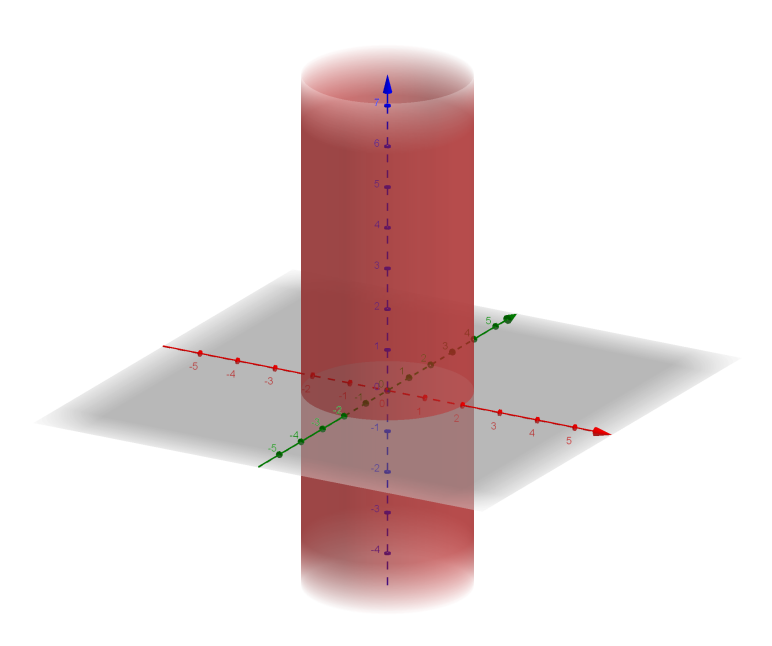
\includegraphics[height = 4cm]{images/second_сylinder.png}
  \end{figure}
\end{example}

\begin{example}
  Пусть линия $\gamma$ представляет собой эллипс, лежащий в координатной плоскости $Oxz$ и задаваемый каноническим уравнением $\frac{x^2}{a^2} + \frac{z^2}{c^2} = 1$.

  Чтобы составить уравнение поверхности, получаемой вращением этого эллипса вокруг оси $Ox$, надо разрешить уравнение относительно $z$: $$
    z = \pm c \sqrt{1 - \frac{x^2}{a^2}}
  $$
  
  Тогда уравнение поверхности вращения имеет вид:$$
    y^2 + z^2 = (\pm \sqrt{1 - \frac{x^2}{a^2}})^2 \Leftrightarrow y^2 + z^2 = c^2(1 - \frac{x^2}{a^2}) \Leftrightarrow \frac{x^2}{a^2} + \frac{y^2}{c^2} + \frac{z^2}{c^2} = 1.
  $$

  Если данный эллипс вращается вокруг оси $Oz$, то уравнение эллипса нужно разрешить относительно
  $x$ и прийти к следующему уравнению поверхности вращения: $$
    \frac{x^2}{a^2} + \frac{y^2}{a^2} + \frac{z^2}{c^2} = 1
  $$
  
  Каждая из этих поверхностей называется эллипсоидом вращения.
  \begin{figure}[H]
    \centering
    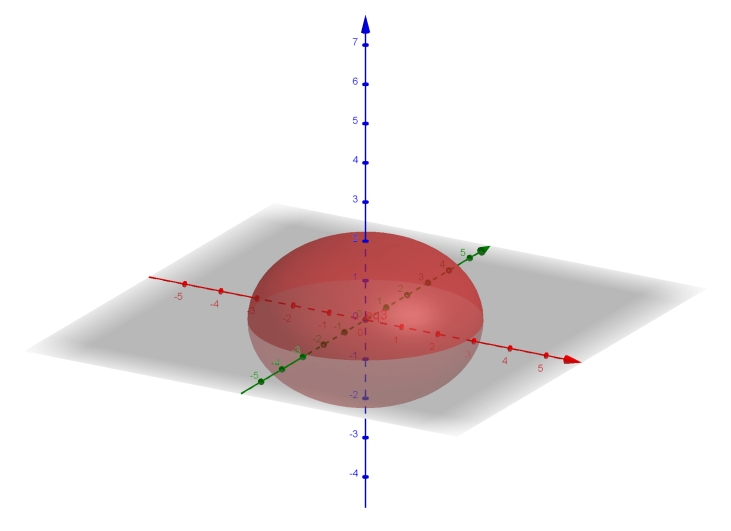
\includegraphics[height = 4cm]{images/second_ellipsoid.png}
  \end{figure}
\end{example}

\subsection*{Конические поверхности}

Рассмотрим поверхность, определяемую в некоторой декартовой системе координат уравнением $F(x, y, z)=0$. Если точка $M$ с координатами
$(x, y, z)$ принадлежит поверхности, то при любом $\lambda$ точка $P(\lambda x, \lambda y, \lambda z)$ также принадлежит поверхности.
\begin{definition}
  Поверхность, которая состоит из прямых линий, проходящих через фиксированную точку, называется \textit{конической поверхностью} или \textit{конусом}. 
  
  Прямые линии называются ее \textit{образующими}, а точка — \textit{вершиной конуса}. 
  
  Линию, лежащую на поверхности, не проходящую
  через вершину и пересекающую все образующие, называют
  \textit{направляющей}.
\end{definition}

\begin{figure}[H]
  \centering
  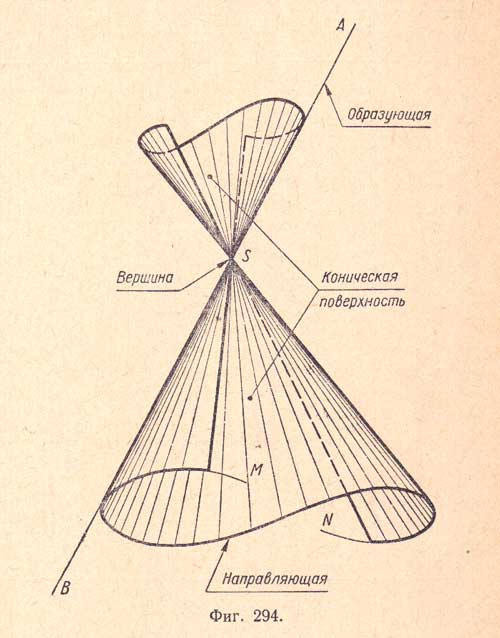
\includegraphics[height = 7cm]{images/second_conical.jpg}
\end{figure}

Напомним уравнение конуса второго порядка: 
$$
  \frac{x^2}{a^2} + \frac{y^2}{b^2} - \frac{z^2}{c^2} = 0, ~ (a \geq b > 0)
$$

\subsection*{Цилиндрические поверхности}

Пусть точка $M_0(x_0, y_0, z_0)$
лежит на поверхности. Тогда все точки с координатами
$x_0, y_0, z$ при любых $z$ также
лежат на поверхности. 
\begin{definition}
  Поверхность, которая состоит из прямых линий, параллельных заданному направлению, называется \textit{цилиндрической поверхностью} или \textit{цилиндром}, а прямые линии — ее \textit{образующими}.
  
  Линию, лежащую на поверхности и пересекающую все образующие, называют \textit{направляющей}.
\end{definition}

\begin{figure}[H]
  \centering
  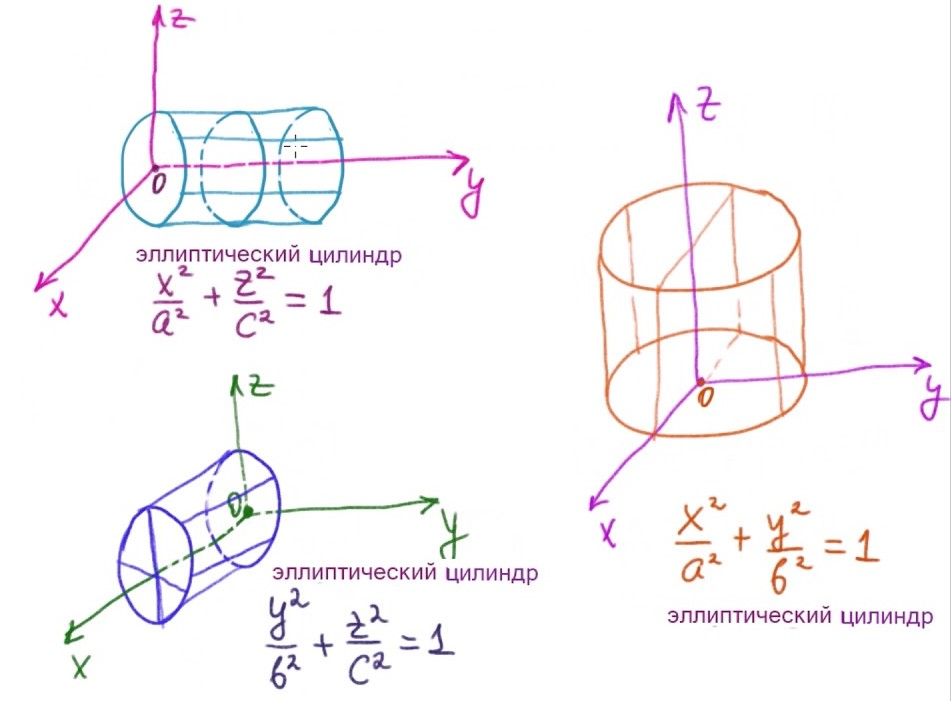
\includegraphics[height = 6cm]{images/second_cylinder_surface.jpg}
\end{figure}

\subsection*{Эллипсоид}
Поверхность с уравнением $$
  \frac{x^2}{a^2} + \frac{y^2}{b^2} + \frac{z^2}{c^2} = 1
$$ называется эллипсоидом.

Эллипсоид получается вращением эллипсоида вдоль малой оси эллипса либо большой оси.
\begin{figure}[H]
  \centering
  \begin{subfigure}[b]{0.4\textwidth}
    \centering
    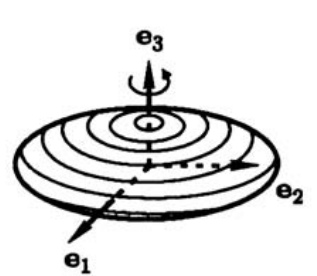
\includegraphics[width = \textwidth]{images/second_ellipsoid_A.png}
  \end{subfigure}
  \hfill
  \begin{subfigure}[b]{0.4\textwidth}
    \centering
    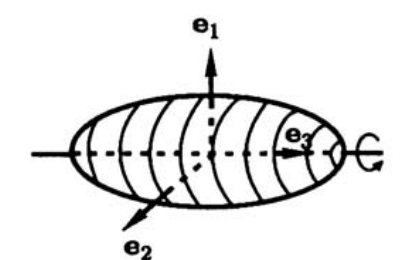
\includegraphics[width = \textwidth]{images/second_ellipsoid_B.png}
  \end{subfigure}
\end{figure}

\subsection*{Однополостный гиперболоид}

Однополостный гиперболоид вращения "--- это поверхность вращения гиперболы вокруг той оси, которая ее не пересекает.
\begin{figure}[H]
  \centering
  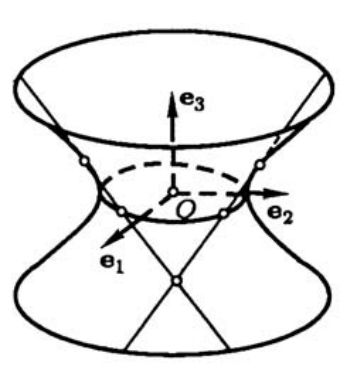
\includegraphics[height = 4cm]{images/second_hyperboloid_one.png}
\end{figure}
Интересное свойство однополостного гиперболоида — наличие у него \textit{прямолинейных образующих}. Так называются прямые линии, всеми своими точками лежащие на поверхности. Через каждую точку однополостного гиперболоида проходят две прямолинейные образующие, уравнения которых можно получить следующим образом. Уравнения этих образующих следующие: $$
  x + y = 1 - z, ~~ x - y = 1 - z. 
$$

Если вместе с гиперболой мы будем вращать ее асимптоты, то они опишут прямой круговой конус, называемый \textit{асимптотическим конусом} гиперболоида вращения.

\subsection*{Двуполостный гиперболоид}
Двуполостный гиперболоид вращения — это поверхность получаемая вращением
гиперболы вокруг той оси, которая ее пересекает.
\begin{figure}[H]
  \centering
  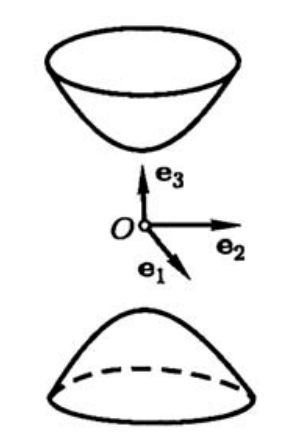
\includegraphics[height = 4cm]{images/second_hyperboloid_two.png}
\end{figure}

\subsection*{Эллиптический параболоид}
Вращая параболу $x^2 = 2pz$ вокруг ее
оси симметрии, мы получаем поверхность, которая называется эллиптическим параболоидом.
\begin{figure}[H]
  \centering
  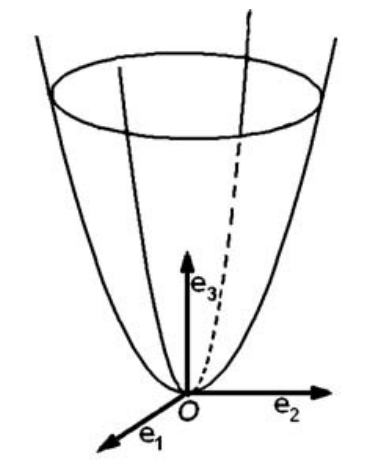
\includegraphics[height = 4cm]{images/second_ellipsoid_parabola.png}
\end{figure}

\subsection*{Гиперболический параболоид}
Поверхность с уравнением $$
  \frac{x^2}{p} - \frac{y^2}{q} = 2z, ~ (p \geq q > 0).
$$
\begin{figure}[H]
  \centering
  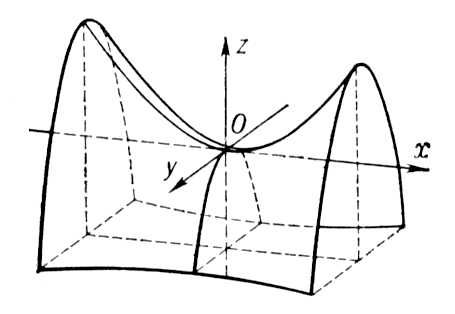
\includegraphics[height = 4cm]{images/second_hyperboloid_parabola.jpg}
\end{figure}

Построить гиперболический параболоид можно
следующим образом: зададим две параболы и будем перемещать одну из них так, чтобы ее вершина скользила по другой, оси парабол были параллельны, параболы лежали во взаимно перпендикулярных плоскостях и ветви их были направлены в противоположные стороны. При таком перемещении
подвижная парабола описывает гиперболический параболоид

Гиперболический параболоид, как и однополостный гиперболоид, имеет два семейства прямолинейных образующих. Уравнения одного семейства $$
  \lambda (\frac{x}{a} - \frac{y}{b}) = \mu, ~~ \mu (\frac{x}{a} + \frac{y}{b}) = 2\lambda z,
$$
а другого  $$
  \lambda'(\frac{x}{a} + \frac{y}{b}) = \mu'. ~~
  \mu'(\frac{x}{a} - \frac{y}{b}) = 2\lambda'z,
$$ "--- где $\lambda$ и $\mu$ произвольные параметры.

\subsection*{Приведение общего уравнения второго порядка на плоскости и в пространстве к каноническому виду}
(если будет выполнено домашнее задание, этот вопрос не нужно учить)

404